\date{}
\title{}
\date{}
\begin{document}
\begin{frame}
    \titlepage
\end{frame}

\input{../common/listingsLib}

\usepgflibrary{shapes.gates.logic.mux}
\newcommand{\z}[2]{\only<#1->{\myemph<#1>{#2}}}
\newcommand{\zz}[3]{\only<#1-#2>{\myemph<#1>{#3}}}
\newcommand{\zzx}[3]{\only<#1-#2>{#3}}
\newlength{\oneZero}
\settowidth{\oneZero}{\small\tt 0}
\newlength{\twoZeroes}
\settowidth{\twoZeroes}{\small\tt 00}



\begin{frame}
\frametitle{last time}
\begin{itemize}
    \item accessing page tables in memory
    \item `fat' tree-based page table data structure
    \item divide virtual page number into parts
    \item repeated table lookup using those parts
        \begin{itemize}
        \item most significant to least significant
        \item physical page number = location of next table (till last part)
        \end{itemize}
    \item view of multi-level lookup as repeated array lookups
\end{itemize}
\end{frame}

\section{virtual memory con't}
\subsection{exercises: multi-level lookup}
% FIXME: \subsubsection{part 0}
% FIXME: \input{../vm/multiSplitExPt0}
\subsubsection{part 2}
\usetikzlibrary{matrix,positioning}

\begin{frame}{2-level splitting}
    \begin{itemize}
    \item 9-bit virtual address 
    \item 6-bit physical address
    \item<2-> \myemph<2>{8-byte pages $\rightarrow$ 3-bit page offset (bottom)}
    \item<2-> 9-bit VA: 6 bit VPN + 3 bit PO
    \item<2-> 6-bit PA: 3 bit PPN + 3 bit PO
    \item<3-> \myemph<3>{1 page page tables w/ 1 byte entry $\rightarrow$ 8 entry PTs}
    \item<4-> \myemph<4>{8 entry page tables $\rightarrow$ 3-bit VPN parts}
    \item<4-> 9-bit VA: 3 bit VPN part 1; 3 bit VPN part 2
    \end{itemize}
\begin{tikzpicture}[overlay,remember picture]
    \coordinate (begin) at ([xshift=-1cm,yshift=-2cm]current page.north east);
    \tikzset{
        page offset/.style={alt=<2>{draw=red,fill=red!10}},
    }
    \begin{scope}[shift={(begin)},x=1.25cm] 
        \draw (-6, 0) rectangle (0, 0.5);
        \node[anchor=south] at (-3, 0.4) {virtual addr};
        \begin{visibleenv}<2-3>
        \draw (-6, 0) rectangle (-2, 0.5) node[midway] {VPN};
        \end{visibleenv}
        \begin{visibleenv}<4->
        \draw (-6, 0) rectangle (-2, 0.5);
            \draw[alt=<4>{red},dotted] (-6, 0) rectangle (-4, 0.5) node[midway,font=\fontsize{11}{12}\selectfont] {VPN pt 1};
            \draw[alt=<4>{red},dotted] (-4, 0) rectangle (-2, 0.5) node[midway,font=\fontsize{11}{12}\selectfont] {VPN pt 2};
        \end{visibleenv}
        \begin{visibleenv}<2->
        \draw[page offset] (-2, 0) rectangle (0, 0.5) node[midway] {page offset};
        \end{visibleenv}
        \begin{scope}[every node/.style={font=\fontsize{10}{11}\selectfont\tt,inner sep=0mm}]
            \node[anchor=north] at (0, 0) {0};
            \node[anchor=north] at (-2, 0) {3};
            \node[anchor=north] at (-4, 0) {6};
            \node[anchor=north] at (-6, 0) {9};
        \end{scope}
        \begin{scope}[yshift=-1.5cm]
            \draw (-4, 0) rectangle (0, 0.5);
            \node[anchor=south] at (-2, 0.4) {physical addr};
            \begin{visibleenv}<2->
            \draw (-4, 0) rectangle (-2, 0.5) node[midway] {PPN};
            \draw[page offset] (-2, 0) rectangle (0, 0.5) node[midway] {page offset};
            \end{visibleenv}
            \begin{scope}[every node/.style={font=\fontsize{10}{11}\selectfont\tt,inner sep=0mm}]
                \node[anchor=north] at (0, 0) {0};
                \node[anchor=north] at (-2, 0) {3};
                \node[anchor=north] at (-4, 0) {6};
            \end{scope}
        \end{scope}
        \begin{visibleenv}<3->
        \begin{scope}[yshift=-4cm]
            \matrix[tight matrix,
                nodes={text width=1cm,font=\small},
                column 1/.style={nodes={text width=0.6cm,draw=none}},
                row 1/.style={nodes={draw=none}},
                label={north:page table \small (either level)},
            ] at (-1, 0){
                ~ \& valid? \& PPN \\
                0 \& ~ \& ~ \\
                1 \& ~ \& ~ \\
                2 \& ~ \& ~ \\
                \ldots \& |[draw=none]|\ldots \& |[draw=none]|\ldots \\
                \myemph<4>{7} \& ~ \& ~ \\
            };
        \end{scope}
        \end{visibleenv}
    \end{scope}
\end{tikzpicture}
\end{frame}

\begin{frame}{2-level example}
\begin{itemize}
\item {}\myemph<1>{9-bit} virtual addresses, 6-bit physical; 8 byte pages, 1 byte PTE
\item page tables 1 page; PTE: 3 bit PPN (MSB), 1 valid bit, 4 unused
\item page table base register {\tt 0x20}; translate virtual address {\tt 0x129}
\end{itemize}
\begin{tikzpicture}
\matrix[tight matrix,anchor=north west,
    nodes={text width=2cm,minimum height=0.5cm,font=\small},
    column 1/.style={nodes={draw=none,font=\small\tt,align=right}},
    column 2/.style={nodes={draw,thick,font=\small\tt,text width=2.6cm,align=left}},
    row 1/.style={nodes={draw=none,font=\small\normalfont}},
    ] (memA)  {
    physical addresses \& bytes \\
    0x00-3 \& 00 11 22 33 \\
    0x04-7 \& 44 55 66 77 \\
    0x08-B \& 88 99 AA BB \\
    0x0C-F \& CC DD EE FF \\
    0x10-3 \& 1A 2A 3A 4A \\
    0x14-7 \& 1B 2B 3B 4B \\
    0x18-B \& 1C 2C 3C 4C \\
    0x1C-F \& 1C 2C 3C 4C \\
};
\matrix[tight matrix,anchor=north west,
    nodes={text width=2cm,minimum height=0.5cm,font=\small},
    column 1/.style={nodes={draw=none,font=\small\tt,align=right}},
    column 2/.style={nodes={draw,thick,font=\small\tt,text width=2.6cm,align=left}},
    row 1/.style={nodes={draw=none,font=\normalfont\small}},
    ] (memB) at ([xshift=0cm]memA.north east) {
    physical addresses \& bytes \\
    0x20-3 \& 00 91 72 13 \\
    0x24-7 \& \maybeEmph<2>{F4} A5 36 07 \\
    0x28-B \& 89 9A AB BC \\
    0x2C-F \& CD DE EF F0 \\
    0x30-3 \& BA \maybeEmph<5>{0A} BA 0A \\
    0x34-7 \& DB 0B DB 0B \\
    0x38-B \& EC 0C EC 0C \\
    0x3C-F \& AC \maybeEmph<3>{DC} DC 0C \\
};
\iftoggle{heldback}{}{
\begin{visibleenv}<2->
\node[right=0cm of memB,align=left,font=\small] {
    {\tt 0x129} = {\tt \myemph<2>{\color<6>{blue}1 00}\myemph<3>{\color<6>{violet}10 1}\myemph<5>{\color<6>{orange}001}} \\
    \texttt{0x20} + {\color<6>{blue}\tt 0x4}~\times 1 = {\tt 0x24} \\
    \textit{PTE 1 value:} \\
    {\tt 0xF4} = {\tt 1111 0100} \\
    PPN {\tt {\color<6>{green} 111}}, valid {\tt 1} \\
    \only<3->{\textit{PTE 2 addr:}} \\
    \only<3->{\texttt{{\color<6>{green} 111} 000} +  \texttt{\myemph<3>{\color<6>{violet} 101}} $\times$ 1 = {\tt 0x3D}}\\
    \only<3->{\textit{PTE 2 value:} {\tt 0xDC}} \\
    \only<4->{PPN {\tt \myemph<4>{\color<6>{red}110}}; valid {\tt 1}} \\
    \only<4->{M[\texttt{\myemph<4>{\color<6>{red}110} \myemph<5>{\color<6>{orange}001}} (\texttt{0x31})] = \texttt{0x0A}}
};
\end{visibleenv}
}
\end{tikzpicture}
\end{frame}

\subsubsection{part 3}
\input{../vm/multiSplitExPt3}
\input{../vm/multiSplitExPt3b}
\subsubsection{part 4}
\input{../vm/multiSplitExPt4}
\subsubsection{part 5}
\input{../vm/multiSplitExPt5}

\section{caching}

\subsection{memory hierarchy intro}
\input{../caching/memHierarchyIntro}

\subsection{locality}
\input{../caching/localityBasics}

\subsection{direct mapped caches}
\input{../caching/directMappedIntro}

\begin{frame}{terminology}
    \begin{itemize}
    \item row = set
        \begin{itemize}
        \item preview: change how much is in a row
        \end{itemize}
    \end{itemize}
\end{frame}

\subsection{tag/index/offset for direct mapped caches}
\input{../caching/tioDMIntro}

\subsection{tio for DM: exercise}
\input{../caching/tioDmExercise}

\subsection{simulating a direct mapped cache}
\input{../caching/dmExampleAccess}

\subsection{exercise: direct-mapped cache access}
\input{../caching/dmAccessExercise}

\subsection{on split data/instruction caches and hierarchy}
\usetikzlibrary{arrows.meta,calc,patterns}

\begin{frame}{split caches; multiple cores}
\begin{tikzpicture}
    \tikzset{
        >=Latex,
        connect/.style={<->,ultra thick},
        cache/.style={draw,very thick,align=center},
    }
\node[cache] (icache1) {instr. \\ cache \\ (core 1)};
\node[cache,anchor=west] (dcache1) at ([xshift=2cm]icache1.east) {data \\ cache \\ (core 1)};
\node[cache] (icache2) {instr. \\ cache \\ (core 1)};
\node[cache,anchor=west] (icache2) at ([xshift=3cm]dcache1.east) {instr. \\ cache \\ (core 2)};
\node[cache,anchor=west] (dcache2) at ([xshift=2cm]icache2.east) {data \\ cache \\ (core 2)};
\node[cache, minimum width=4cm,anchor=north] (l21) at ([yshift=-1cm]$(icache1.south)!0.5!(dcache1.south)$) {unified \\ L2 cache \\ (core 1)};
\node[cache, minimum width=4cm,anchor=north] (l22) at ([yshift=-1cm]$(icache2.south)!0.5!(dcache2.south)$) {unified \\ L2 cache \\ (core 2)};
    \node[cache, minimum width=8cm,anchor=north] (l3) at ([yshift=-1cm]$(l21.south)!0.5!(l22.south)$) {L3 cache \\ (shared between cores)};
\foreach \fromC/\toC in {icache1/l21,dcache1/l21,icache2/l22,dcache2/l22,l21/l3,l22/l3} {
\draw[connect] (\fromC.south) -- ++(-0cm,-.5cm) -| (\toC.north);
}
\end{tikzpicture}
\end{frame}

\begin{frame}{hierarchy and instruction/data caches}
    \begin{itemize}
    \item typically separate data and instruction caches for L1
    \vspace{.5cm}
    \item (almost) never going to read instructions as data or vice-versa
    \item avoids instructions evicting data and vice-versa
    \item can optimize instruction cache for different access pattern
    \item easier to build fast caches: that handles less accesses at a time
    \end{itemize}
\end{frame}



% FIXME: direct-mapped and C code example
\section{misses in C, and intuition behind conflicts}
\input{../caching/conflictMissesAndC}

\section{array misses warmup}
\input{../caching/arrayMissesWarmupEx}

\section{array misses and cache results}
\begin{frame}[fragile,label=arrayMissesOddEven1]{arrays and cache misses (1)}
\begin{lstlisting}
int array[1024]; // 4KB array
int even_sum = 0, odd_sum = 0;
for (int i = 0; i < 1024; i += 2) {
    even_sum += array[i + 0];
    odd_sum +=  array[i + 1];
}
\end{lstlisting}
    \begin{itemize}
        \item {\small
Assume everything but {\tt array} is kept in registers (and the compiler does not do
            anything funny).}
\item
How many \textit{data cache misses} on initially empty 2KB direct-mapped cache with 16B cache blocks?
    \end{itemize}
\end{frame}

\begin{frame}<1>[fragile,label=arrayMissesOddEven2]{arrays and cache misses (2)}
\begin{lstlisting}
int array[1024]; // 4KB array
int even_sum = 0, odd_sum = 0;
for (int i = 0; i < 1024; i += 2)
    even_sum += array[i + 0];
for (int i = 0; i < 1024; i += 2)
    odd_sum +=  array[i + 1];
\end{lstlisting}
    \begin{itemize}
        \item {\small
    Assume everything but {\tt array} is kept in registers (and the compiler does not do
    anything funny).
        }
    \item
How many \textit{data cache misses} on initially empty 2KB direct-mapped cache with 16B cache blocks?
            \only<2->{Would a set-associtiave cache be better?}
    \end{itemize}
\end{frame}

\begin{frame}[fragile,label=arrayMissesOddEven3]{arrays and cache misses (2b)}
\begin{lstlisting}
int array[1024]; // 4KB array
int even_sum = 0, odd_sum = 0;
for (int i = 0; i < 1024; i += 2)
    even_sum += array[i + 0];
for (int i = 0; i < 1024; i += 2)
    odd_sum +=  array[i + 1];
\end{lstlisting}
    \begin{itemize}
        \item {\small
    Assume everything but {\tt array} is kept in registers (and the compiler does not do
    anything funny).
        }
    \item
        How many \textit{data cache misses} on initially empty \myemph{4KB} direct-mapped cache with 16B cache blocks?
    \end{itemize}
\end{frame}

\begin{frame}[fragile,label=arrayMisses4]{arrays and cache misses (3)}
\begin{lstlisting}
int array[1024]; // 4KB array
int sum;
for (int i = 8; i < 1016; i += 1) {
    int local_sum = 0;
    for (int j = i - 8; j < i + 8; j += 1) {
        local_sum += array[i] * (j - i);
    }
    sum += (local_sum - array[i]);
}
\end{lstlisting}
    \begin{itemize}
        \item {\small
    Assume everything but {\tt array} is kept in registers (and the compiler does not do
    anything funny).
        }
    \item
        How many \textit{data cache misses} on initially empty \myemph{2KB} direct-mapped cache with 16B cache blocks?
    \end{itemize}
\end{frame}



\section{cache misses on more complex code}
\begin{frame}{actual misses: BST lookups}
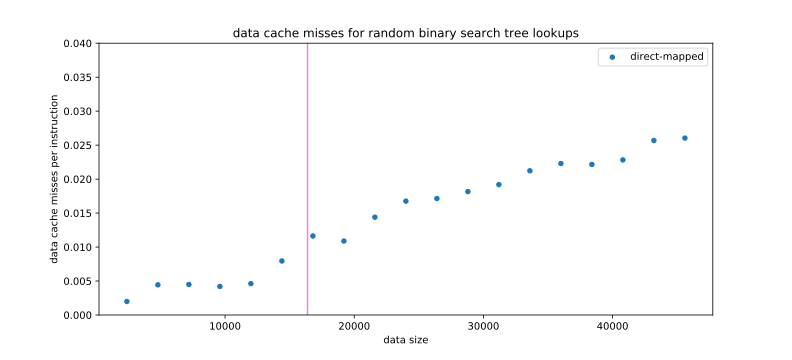
\includegraphics[width=\textwidth]{../caching/bst-one}
\end{frame}

\begin{frame}{actual misses: matrix multiplies}
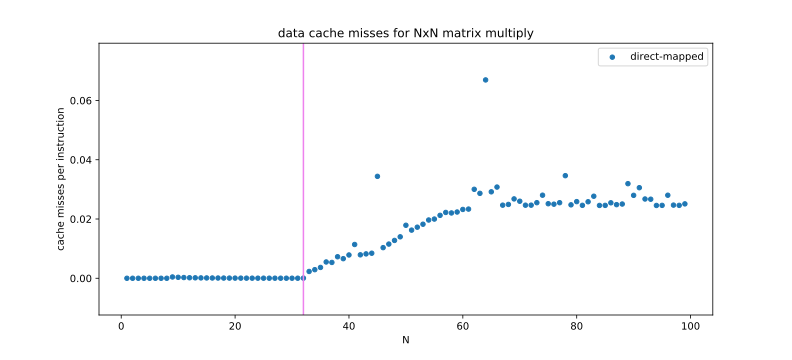
\includegraphics[width=\textwidth]{../caching/mm-one}
\end{frame}


\section{array misses and skipping around}
\begin{frame}<1>[fragile,label=arrayMissesSkip]{misses with skipping}
\begin{lstlisting}
int array1[512]; int array2[512];
...
for (int i = 0; i < 512; i += 1)
    sum += array1[i] * array2[i];
}
\end{lstlisting}
    \begin{itemize}
        \item {\small
    Assume everything but {\tt array1}, {\tt array2} is kept in registers (and the compiler does not do
    anything funny).
        }
    \item
About how many \textit{data cache misses} on a 2KB direct-mapped cache with 16B cache blocks? \\
Hint: depends on relative placement of array1, array2
\end{itemize}
\end{frame}

\begin{frame}{best/worst case}
\begin{itemize}
\item \texttt{array1[i]} and \texttt{array2[i]} always different sets:
    \begin{itemize}
    \item 2 misses every 4 \texttt{i}
    \item = distance from array1 to array2 not multiple of \# sets $\times$ bytes/set
    \end{itemize}
\item \texttt{array1[i]} and \texttt{array2[i]} same sets:
    \begin{itemize}
    \item 2 misses every \texttt{i}
    \item = distance from array1 to array2 is multiple of \# sets $\times$ bytes/set
    \end{itemize}
\end{itemize}
\end{frame}

\begin{frame}{worst case in practice?}
    \begin{itemize}
    \item two rows of matrix?
    \item often sizeof(row) bytes apart
    \item if the row size is multiple of number of sets $\times$ bytes per block, oops!
    \end{itemize}
\end{frame}


\subsection{adding associativity}
\againframe<13>{pattern1}

\input{../caching/addAssoc}

\subsection{associativity terms}
\input{../caching/assocTerms}

\subsection{tag/index/offset for set-assoc. caches}
\begin{frame}{Tag-Index-Offset formulas}
\def\arraystretch{1.5}
\begin{tabular}{ll}
$m$ & memory addreses bits \\
$E$ & number of blocks per set (``ways'') \\
$S=2^s$ & number of sets \\
$s$  & (set) index bits \\
$B=2^b$ & block size \\
$b$ & (block) offset bits \\
$t = m - (s+b)$ & tag bits \\
$C = B \times S \times E$ & cache size (excluding metadata) \\
\end{tabular}
\end{frame}


\subsection{tag/index/offset exercise}
\subsubsection{setup}
\input{../caching/tioExerciseIntro}
\subsubsection{the exercise}
\input{../caching/tioExercise}

\section{fixing actual misses}
\begin{frame}{simulated misses: BST lookups}
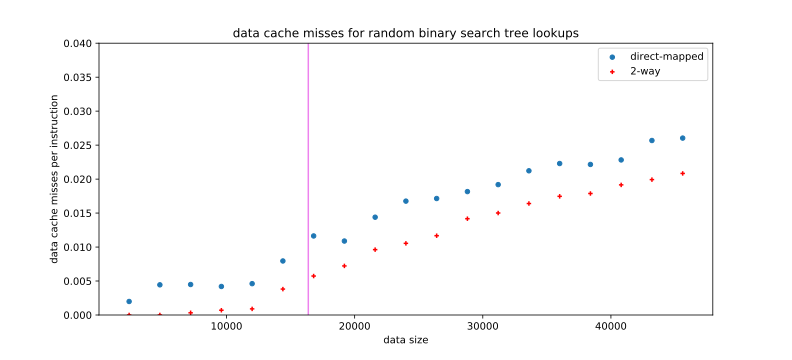
\includegraphics[width=\textwidth]{../caching/bst-both}
\end{frame}

\begin{frame}{simulated misses: matrix multiplies}
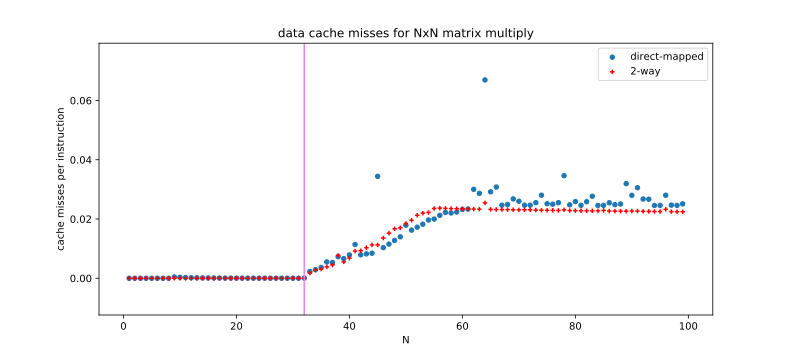
\includegraphics[width=\textwidth]{../caching/mm-both}
\end{frame}


\section{array misses warmup, round 2}

\begin{frame}[fragile,label=arrayMissesWarmup4]{C and cache misses (warmup 4)}
\begin{lstlisting}[style=smaller]
int array[8];
...
int even_sum = 0, odd_sum = 0;
even_sum += array[0];
even_sum += array[2];
even_sum += array[4];
even_sum += array[6];
odd_sum += array[1];
odd_sum += array[3];
odd_sum += array[5];
odd_sum += array[7];
\end{lstlisting}
\begin{itemize}
\item {\small
Assume everything but {\tt array} is kept in registers (and the compiler does not do
anything funny).}
\item How many data cache misses on a \textbf{2}-set direct-mapped cache with 8B blocks?
\end{itemize}
\end{frame}

\begin{frame}<0>[fragile,label=arrayMissesWarmup4Answers]{exercise solution}
\newcommand{\mywidth}{0.39}
\begin{tikzpicture}
    \foreach \offset in {-2,-1,0,1,2,...,31,32,33} {
        \draw[black!25,thin] (\offset * \mywidth, 0) rectangle ++(\mywidth, -1);
    }
    \node[font=\large,anchor=east] at (-2 * \mywidth, -.5) {\ldots};
    \node[font=\large,anchor=west] at (34 * \mywidth, -.5) {\ldots};
    \begin{scope}
    \clip (-2.1 * \mywidth, .2) rectangle (34.1 * \mywidth, -1.1);
    \foreach \offset/\name in {8/0,12/1,16/2,20/3,24/4,28/5,32/6} {
        \draw[thin,fill=blue!10] (\offset * \mywidth, 0) rectangle ++(\mywidth * 4, -1)
            node[fill=none,opacity=1.0,black,midway,font=\fontsize{9}{10}\tt\selectfont] {array[\name]};
    }
    \foreach \offset in {-8,0,8,16,24,32} {
        \draw[ultra thick,red!30!black] (\offset * \mywidth, 0)
            rectangle ++(\mywidth * 8, -1);
    }
    \end{scope}
        \draw[very thick, decorate, decoration={brace}] (8 * \mywidth, 0.05) -- ++(8 * \mywidth, 0)
            node[above,midway,align=center,font=\small] {one cache block \\
                                (index 0)};
        \draw[very thick, decorate, decoration={brace}] (16 * \mywidth, 0.05) -- ++(8 * \mywidth, 0)
            node[above,midway,align=center,font=\small] {one cache block \\
                                (index 1)};
        \draw[very thick, decorate, decoration={brace}] (24 * \mywidth, 0.05) -- ++(8 * \mywidth, 0)
            node[above,midway,align=center,font=\small] {one cache block \\
                                (index 0)};
        \draw[very thick, decorate, decoration={brace}] (0 * \mywidth, 0.05) -- ++(8 * \mywidth, 0)
            node[above,midway,align=center,font=\small] {one cache block \\
                                (index 1)};
    \tikzset{
        set both/.style={alt=<2-3>{nodes={fill=red!10}}},
        set 0/.style={
            alt=<2>{nodes={fill=red!10}},
            alt=<3>{opacity=0.1},
        },
        set 1/.style={
            alt=<3>{nodes={fill=red!10}},
            alt=<2>{opacity=0.1},
        },
    }
    \matrix[tight matrix,
        nodes={minimum height=0.5cm,font=\fontsize{8}{9}\selectfont},
        column 1/.append style={nodes={text width=4cm}},
        column 2/.append style={nodes={text width=5cm,font=\fontsize{10}{11}\tt\selectfont,set 0}},
        column 3/.append style={nodes={text width=5cm,font=\fontsize{10}{11}\tt\selectfont,set 1}},
        row 1/.append style={nodes={font=\fontsize{9}{10}\bfseries\selectfont}},
        row 2/.append style={set both},
        row 3/.append style={set 0},
        row 4/.append style={set 1},
        row 5/.append style={set 0},
        row 6/.append style={set 1},
        row 7/.append style={set 0},
        row 8/.append style={set 1},
        row 9/.append style={set 0},
        row 10/.append style={set 1},
        anchor=north west] at (-1, -1) {
        memory access \& set 0 afterwards \& set 1 afterwards \\ 
        --- \& (empty) \& (empty) \\
        read \lstinline|array[0]| (miss) \& \{array[0], array[1]\} \& (empty) \\
        read \lstinline|array[2]| (miss) \& \{array[0], array[1]\} \& \{array[2], array[3]\} \\
        read \lstinline|array[4]| (miss) \& \{array[4], array[5]\} \& \{array[2], array[3]\} \\
        read \lstinline|array[6]| (miss) \& \{array[4], array[5]\} \& \{array[6], array[7]\} \\
        read \lstinline|array[1]| (miss) \& \{array[0], array[1]\} \& \{array[6], array[7]\} \\
        read \lstinline|array[3]| (miss) \& \{array[0], array[1]\} \& \{array[2], array[3]\} \\
        read \lstinline|array[5]| (miss) \& \{array[4], array[5]\} \& \{array[2], array[3]\} \\
        read \lstinline|array[7]| (miss) \& \{array[4], array[5]\} \& \{array[6], array[7]\} \\
    };
\end{tikzpicture}
\end{frame}

\iftoggle{heldback}{}{
\againframe<1-3>{arrayMissesWarmup4Answers}
}


\againframe<2>{arrayMissesOddEven2}

\subsection{options for replacement}
\input{../caching/replacement}

\subsection{options for handling writes}
\input{../caching/writePolicy}
% FIXME: writes and what counts as a miss

\subsection{exercise: write/replacement policies}
\input{../caching/writeReplaceExercise}

\subsection{fast writes: write buffers}
\input{../caching/fastWrites}

\subsection{miss types}
\begin{frame}{cache miss types}
    \begin{itemize}
        \item common to categorize misses:
            \begin{itemize}
            \item roughly ``cause'' of miss assuming cache block size fixed
            \end{itemize}
        \vspace{.5cm}
        \item \textit{compulsory} (or \textit{cold}) --- \myemph{first time} accessing something
            \begin{itemize}
            \item adding more sets or blocks/set wouldn't change
            \end{itemize}
        \item \textit{conflict} --- sets aren't big/flexible enough
            \begin{itemize}
            \item a fully-associtive (1-set) cache of the same size would have done better
            \end{itemize}
        \item \textit{capacity} --- cache was not big enough
    \end{itemize}
\end{frame}


\section{cache tradeoffs}
\input{../caching/cacheTradeoffs}

\section{TLB}
\subsection{why cache page table entries?}
\input{../caching/tlbWhy}

\subsection{how TLB fits in page table lookup}
\input{../caching/tlbMulti}

\subsection{how TLBs are organized}
\input{../caching/tlbOrganization} % FIXME: emphasize that AFTER this is normal cache access

\subsection{exercise: splitting for TLBs}
\subsubsection{1}
\input{../caching/tlbSplitEx1}
\subsubsection{2}
\input{../caching/tlbSplitEx2}


\subsection{exercise: TLB access pattern}
\input{../caching/tlbAccessExPrep}
\input{../caching/tlbAccessEx}


\subsection{TLBs and context switches}
\input{../caching/tlbSwitch}

\section{backup slides --- general}

\subsection{inclusive v exclusive}
\usetikzlibrary{patterns}
\begin{frame}{inclusive versus exclusive}
\begin{tikzpicture}
\tikzset{
    >=Latex,
    connect/.style={<->,ultra thick},
    cache/.style={draw,very thick},
    fill 1/.style={pattern color=blue!50!black,pattern=crosshatch},
    fill 2/.style={pattern color=orange,pattern=dots},
}
\node (l2 incl label) at (2.5, 6.5) {L2 inclusive of L1};
\node[font=\small,anchor=north,align=center] at (l2 incl label.south) {
    everything in L1 cache duplicated in L2 \\
    adding to L1 also adds to L2
};
\node[anchor=south]  at (1, 2) {L1 cache};
\node[anchor=south]  at (4, 4) {L2 cache};
\draw[cache] (0, 0) rectangle ++(2, 2);
\path[fill 1] (0, 0) rectangle ++(2, 2);
\path[fill 2] (3, -1.5) rectangle ++(2,1);
\path[fill 1] (3, -0.5) rectangle ++(2, .5);
\path[fill 2] (3, 0) rectangle ++(2,.25);
\path[fill 1] (3, 0.25) rectangle ++(2, .3);
\path[fill 2] (3, 0.55) rectangle ++(2,.65);
\path[fill 1] (3, 1.2) rectangle ++(2, .6);
\path[fill 2] (3, 1.8) rectangle ++(2,.2);
\path[fill 1] (3, 2) rectangle ++(2, .6);
\path[fill 2] (3, 2.6) rectangle ++(2,1.4);
\draw[cache] (3, -1.5) rectangle ++(2, 5.5);

\begin{scope}[xshift=8cm]
\node (l2 excl label) at (2.5, 6.5) {L2 exclusive of L1};
\node[font=\small,anchor=north,align=center] at (l2 excl label.south) {
    L2 contains different data than L1 \\
    adding to L1 must remove from L2 \\
    probably evicting from L1 adds to L2
};
\node[anchor=south]  at (1, 2) {L1 cache};
\node[anchor=south]  at (4, 4) {L2 cache};
\path[fill 1] (0, 0) rectangle ++(2, 2);
\draw[cache] (0, 0) rectangle ++(2, 2);
\draw[cache,fill 2] (3, -1.5) rectangle ++(2, 5.5);
\end{scope}
\begin{visibleenv}<2>
    \draw[overlay,red,very thick] (-1,-1.75) rectangle (6.25, 7);
    \fill[fill opacity=0.95,fill=white] (6.75, -1.75) rectangle (14, 7)
        node[midway,align=left,font=\small] {
            inclusive policy: \\
            no extra work on eviction \\
            but duplicated data \\
            ~ \\
            easier to explain when \\
            L$k$ shared by multiple L$(k-1)$ caches?
        };
\end{visibleenv}
\begin{visibleenv}<3>
    \draw[overlay,red,very thick] (6.75, -1.75) rectangle (14, 7);
    \fill[fill opacity=0.95,fill=white](-1,-1.75) rectangle (6.25, 7)
        node[midway,align=left,font=\small] {
            exclusive policy: \\
            avoid duplicated data \\
            sometimes called \textit{victim cache} \\
            (contains cache eviction victims) \\
            ~ \\
            makes less sense with multicore
        };
\end{visibleenv}
\end{tikzpicture}
\end{frame}



\subsection{tag/index/offset formulas}
\begin{frame}{Tag-Index-Offset formulas (direct-mapped only)}
\def\arraystretch{1.5}
\begin{tabular}{ll}
$m$ & memory addreses bits \\
$S=2^s$ & number of sets \\
$s$  & (set) index bits \\
$B=2^b$ & block size \\
$b$ & (block) offset bits \\
$t = m - (s+b)$ & tag bits \\
$C = B \times S$ & cache size (if direct-mapped) \\
\end{tabular}
\end{frame}


\section{backup slides --- cache performance}
\begin{frame}{backup slides --- cache performance}
\end{frame}

\section{AMAT}
\input{../caching/amatFormula}

\subsection{exercise: AMAT (simple case)}
\input{../caching/amatEx}

\subsection{exercise: multi-level cache AMAT}
\input{../caching/multiLevelAMAT}

\section{less precise approxmation}
\input{../caching/approxMisses}

% FIXME: cache performance intro
\section{warmup: locality exercise}  % FIXME: move earlier?
\input{../caching/localityExercise}

\section{warmup: miss counting}
\input{../caching/localityExMissCount}

\section{2D arrays in C}
\input{../caching/c2DArray}
% FIXME: cache blocks and 2D array
\input{../caching/2DArrayBlock}

\section{matrix multiply and loop orders}
\input{../caching/matrixMultIntro}
%\input{../caching/matrixSqIntro}
\input{../caching/matrixMultOrders}
\input{../caching/matrixMultOrdersLocality}
\subsection{exercise: which order?}
\input{../caching/matrixMultOrdersEx} % FIXME: input

% FIXME: move unused?
\subsection{locality: diagrams}
\input{../caching/blockDiagMultIjk}
\input{../caching/blockDiagMult}

\subsection{MM performance}
\againframe<2>{matrixMultTwoVersions}
\input{../caching/matrixMultOrdersPerf}

\subsection{miss counting}
\input{../caching/matrixMultOrdersMisses}

\subsection{miss count exericse}
\input{../caching/localityExMissCount2}

\subsection{jagged edges: conflict misses} % FIXME: cut if not time
\input{../caching/matrixMultOrdersConflicts}


\section{warmup, take two: locality exercise}
\input{../caching/localityExercise2}

\section{cache blocking introduction}
%\input{../caching/blockingIntroSq}
\subsection{transformation --- 1D blocking}
\input{../caching/blockingIntroMultXformK}
\subsubsection{missses in A}
\input{../caching/blockingIntroMultKMissesA}
\subsubsection{missses in B}
\input{../caching/blockingIntroMultKMissesB}
\subsubsection{overall misses}
\input{../caching/blockingIntroMultKMissesOverall}
\subsubsection{actual performance}
\input{../caching/blockingIntroMultKReadMissGraph}

\subsection{two-at-a-time}
\input{../caching/blockingIntro2Mult}
%\input{../caching/blockingGeneralSq}
% FIXME: diagram
%\input{../caching/blockingDivideAndConquerSq} % FIXME: earlier?

\subsection{generalizing}
\input{../caching/blockingDivideAndConquerMult}

\subsection{diagram of general}
\input{../caching/blockingUsageGeneralMult}

%\subsection{locality view}
%\input{../caching/blockDiagSq}
%\input{../caching/loopIneff} % FIXME: drop?

\section{counting loads}
%\input{../caching/loadingCountsSq}
\input{../caching/loadingCountsMult}

\section{exercise}
\input{../caching/localityExMissCount3}


\section{cache blocking review}
\input{../caching/cacheBlockingReview} % FIXME: really before arrays and blocks?


\section{backup slides}
\begin{frame}{backup slides}
\end{frame}

% FIXME:
\subsection{cut example?}
\input{../caching/dmExampleAccessCut}

\subsection{benchmarking and cache results}
\input{../caching/cacheBenchExample}


\section{varying parameters exercise}
    % FIXME: put back?
\input{../caching/cacheTradeoffsEx}

\subsection{misc cache optimizations: prefetching}
    % FIXME: put back? (named in tradeoffs table)
\input{../caching/miscCacheOpt}

\subsection{an old quiz question}
\input{../caching/arrayMissesQuizAnswer}

\subsection{mapping misses to sets (DM)}
\input{../caching/setMappingDiagDM}
\subsection{mapping misses to sets (3-way)}
\input{../caching/setMappingDiag3}

\subsection{sparse array miss exericse}
\input{../caching/arrayMissesExSparseConflicts}

\section{alternate cache miss exericse}
\input{../caching/arrayMissesExSparseAlt}

\section{array misses and cache results (old sparse)}
\input{../caching/arrayMissesExSparse}

\subsection{set mapping (text)}
\input{../caching/setMappingText}



\subsection{addt'l order usage diagrams}
\againframe<6->{ijkCacheUsage}
\againframe<6->{kijCacheUsage}

\subsection{cache blocking: more than two at a time?}
\input{../caching/blockingIntroMultKTo3}
%\input{../caching/blockingIntroMult}
\input{../caching/blockingUsageMult}

\subsection{explicit counting}
\input{../caching/explicitCounting}

\subsection{how TLBs fit in the pipeline}
\input{../caching/tlbPipeline}




\section{backup slides}
\begin{frame}{backup slides}
\end{frame}

\end{document}
